\chapter{Introduction}
\label{cha:introduction}

\section{Overview and aims}
%original work
The stratosphere is the layer of the Earth's atmosphere bounded by the
tropopause below and the stratopause above. The height of the tropopause varies
from about 15~km in altitude in the tropics to 7~km at high latitudes, while the
stratopause lies at approximately 50~km. The defining feature of the
stratosphere is a temperature gradient increasing with height (in contrast to
the troposphere below), caused by the presence of ozone which absorbs
ultraviolet radiation\footnote{For this reason, the region of the stratosphere
  with the highest ozone concentrations is often called the ``ozone layer''.}
and thereby heats the surrounding atmosphere. This temperature gradient makes
the stratosphere stable against vertical convection and results in very
different dynamical behaviour to the troposphere.

Traditionally the stratosphere was thought to respond passively to tropospheric
forcing from below. However, modelling and observational evidence accrued over
approximately the last two decades has suggested that in some cases variability
of the winter polar stratosphere can cause consistent circulation anomalies at
the Earth's surface. This influence has been shown to be particularly strong
following the rapid breakdown of the usual westerly winter stratospheric polar
vortex; events known as sudden stratospheric warmings (SSWs). 

Despite these advances, important issues remain as to the dynamics of SSWs
and the stratosphere's influence on the troposphere. Most significantly:
\begin{enumerate}[i.]
\item The dynamics of SSWs are not fully understood, in particular whether
  different mechanisms may be responsible for different types of event.
\item A mechanism for the stratosphere's influence on the troposphere is not
  well developed and is not understood why some types of stratospheric event
  appear to have a larger or different impact on the troposphere than others.
\end{enumerate}
These are large and long-standing issues, and providing a comprehensive solution
is not possible here, but it is hoped that this thesis will go at least some way
to addressing them. A solution to these issues is not purely of theoretical
interest, as it is necessary to understand the dynamics of these phenomena in
order to model them and put them to use in weather and climate predictions. With
an eye on this application, we also aim to assess the predictability of the
stratosphere and its connection to the troposphere in these models.

The main original contributions of this thesis to the scientific literature are
outlined below:
\begin{enumerate}[1.]
\item In \textbf{Chapter \ref{cha:moments}} a new method to diagnose
  stratospheric polar vortex variability and classify split and displaced vortex
  events is introduced and tested. This is the first vortex-centric method that
  can be easily and robustly applied to climate model simulations.

\item In \textbf{Chapter \ref{cha:models}} this method is applied to carry out
  the first multi-model comparison of split and displaced vortex events and
  their influence on the troposphere. It is found that there are a wide range of
  biases among models, at least some of which may be attributable to differences
  in vertical resolution. Furthermore, the large number of events studies allows
  some inference of the mechanisms behind the different surface response to
  split and displaced vortex events. 

\item In \textbf{Chapter \ref{cha:seas}} the preidctability of the stratospheric
  polar vortex is assessed in a stratosphere-resolving seasonal prediction
  system. Little skill is found in the prediction of the strength of Northern
  Hemisphere stratospheric polar vortex or the occurrence of split or displaced
  vortex events on seasonal timescales. However, sigificant skill is found in
  the case of the Southern Hemisphere vortex, allowing for the prediction of
  interannual variability in ozone depletion and with a significant influnce on
  the surface beyond the lead time of previous forecasts. 
\end{enumerate}

In the remainder of this chapter, the necessary background to the dynamics of
the polar stratosphere (Section \ref{sec:dynam-polar-strat}) and its influence
on the troposphere (Section \ref{sec:strat-trop-coupl}) are discussed.

\subsection{Relation to published work}
Chapter \ref{cha:moments} is largely based on a paper written by myself, Daniel
Mitchell and Lesley Gray in \emph{Geophysical Research Letters}
\citep{Seviour2013}, although the analysis has been significantly extended and
re-written. The results in Chapter \ref{cha:seas} on the Southern Hemisphere are
based on a paper written by myself, Steven Hardiman, Lesley Gray, Neal Butchart,
Craig MacLachlan, and Adam Scaife in \emph{Journal of Climate}
\citep{Seviour2014}. 

In both of these papers, all the writing is my own and I carried out all the
analysis and produced the figures. However, I am of course very grateful for the
constructive comments of my coauthors in the preparation of these papers as well
as my reviewers; Harry Hendon (from the Centre for Australian Weather and
Climate Research), and three of whom are anonymous.



\section{Dynamics of the polar stratosphere}
\label{sec:dynam-polar-strat}


\subsection{Zonal mean flow}

Each winter the polar regions descend into a polar night and the stratosphere
cools by infrared radiation to space. This sets up a strong meridional
temperature gradient which increases the vertical zonal wind shear in accordance
with the thermal wind balance relation
\begin{equation}
\frac{\partial u_g}{\partial z} = -\frac{R}{fH}\frac{\partial T}{\partial y} \,, 
\end{equation} 
where $u_g$ is the geostrophic zonal velocity,
$u_g = -f^{-1}\partial Z/\partial y$, $Z$ is geopotential height, $f$ is the
Coriolis parameter, $f=2\Omega\sin\phi$, and $R$ is the specific gas
constant. Here, a beta-plane geometry is used such that $f=f_0+\beta y$, where
$f_0=f(\phi_0)$ and $\beta = 2\Omega a^{-1}\cos\phi_0$, $a$ is the Earth's
radius and $\phi_{0}$ is a reference latitude. $H$ is the scale height given by
$H = RT_s/g$, where $T_s$ is a reference temperature and $g$ is the acceleration
due to gravity. This equation relies on hydrostatic and geostrophic
approximations but is approximately satisfied on seasonal timescales. Hence, the
meridional temperature gradient decreasing from equator to pole results in a
region of westerly winds surrounding the pole; this is known as the
stratospheric polar vortex.

\begin{figure}
 \centering
 \noindent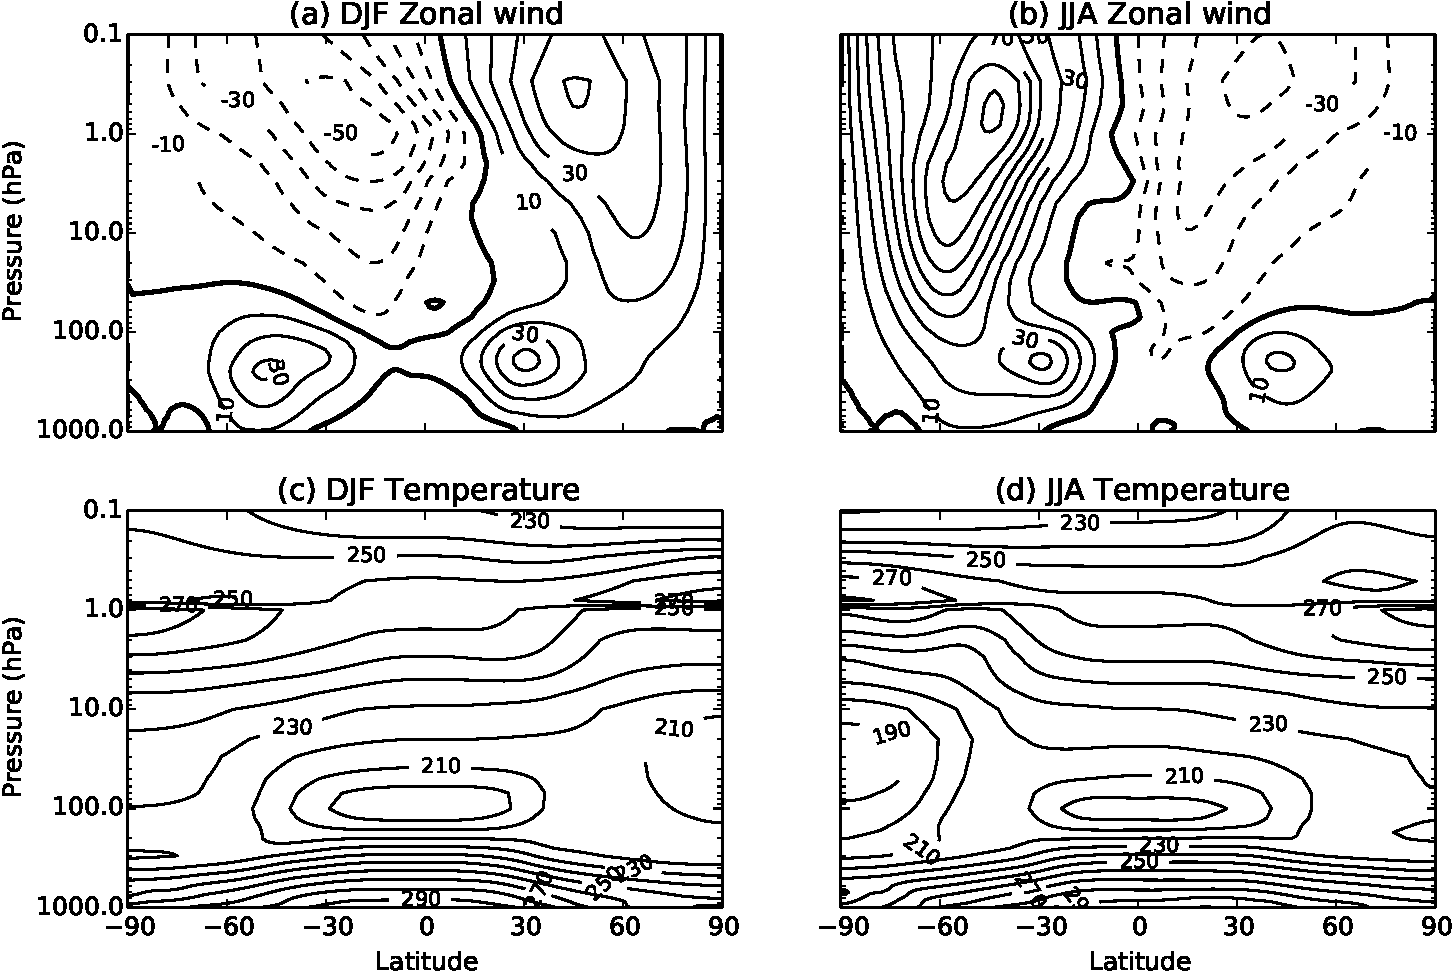
\includegraphics[width=\textwidth]{figures/chapter-intro/zmzw_zmT_clim.pdf}
 \caption[Zonal-mean zonal wind and temperature climatology.]{December-Janurary
   (DJF) (a,c) and July-August (JJA) (b,d) averages of zonal-mean zonal wind
   ($\mathrm{m~s^{-1}}$) (a,b) and temperature (K) (c,d). Data is from the
   ERA-Interim reanalysis (1979-2010).}
 \label{fig:zmzw_zmT_clim}
\end{figure}

Figure \ref{fig:zmzw_zmT_clim} shows zonal-mean zonal wind and temperature
averaged over the boreal winter (December-February; DJF) and austral winter
(July-August; JJA) using data from 1979-2010 from the ERA-Interim reanalysis
(details in Section \ref{sec:reanalysis-data}). In both cases the westerly
vortex in the winter hemisphere can be seen along with a local minimum in
temperature at the winter pole in the lower stratosphere. Weaker easterly winds
are present in the summer hemisphere. The maximum strength of the polar vortex
occurs at midlatitudes between 0.1-1~hPa in the mesosphere, and is stronger in
the Southern Hemisphere (SH) with a maximum of $90~\mathrm{ms^{-1}}$ than the
Northern Hemisphere (NH) with a maximum of $50~\mathrm{ms^{-1}}$. The winter
polar stratosphere is also approximately 20~K colder in th SH than the NH. 

\begin{figure}
 \centering
 \noindent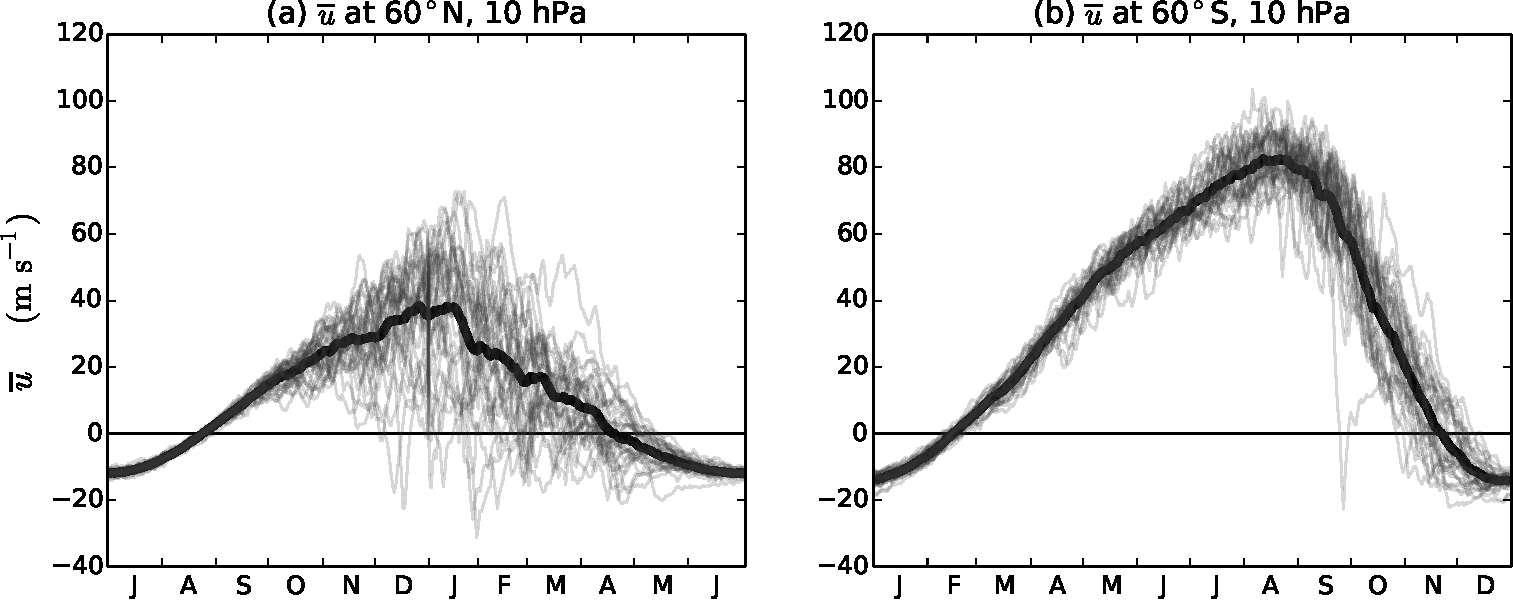
\includegraphics[width=\textwidth]{figures/chapter-intro/zmzw_NH_SH.pdf}
 \caption[Comparison of NH and SH polar vortex seasonal cycle.]{Seasonal cycle
   of NH (a) and SH (b) polar vortex strength, measured by $\overline{u}$ at
   60$^{\circ}$N/S, 10~hPa. The annual mean is shown in a thick black line and
   individual years in thin grey lines. Both time series are centred on their
   respective winters. Data is from the ERA-Interim reanalysis (1979-2009).}
 \label{fig:zmzw_NH_SH}
\end{figure}

The maximum strength of the vortex in the stratosphere occurs at approximately
$60^{\circ}$N/S with little variation through the depth of the
stratosphere. Figure \ref{fig:zmzw_NH_SH} shows the annual cycle and variability
of zonal-mean zonal wind at 10~hPa $60^{\circ}$N and $60^{\circ}$S. As well as
being weaker on average than the SH, the winter NH stratospheric polar vortex
can also be seen to be significantly more variable than the SH. There are a
number of years in the NH for which $\overline{u}$ becomes negative during the
winter, but only one such year in the SH (these events are discussed further in
Section \ref{sec:strat-sudd-warm}). A further clear feature of both NH and SH is
that variability during the summer is much less than that during winter. All
these observations are due almost entirely to the influence of wave phenomena in
the stratosphere, as described in the next section.


\subsection{Waves in the stratosphere}
\label{sec:plan-waves-strat}

\subsubsection{Planetary waves}
\label{sec:planetary-waves}

Large-scale Rossby or planetary waves\footnote{Here, as is common in the
  stratospheric literature, ``wave'' is taken to mean any deviation from the
  zonal-mean state which not necessarily a physical structure.} play a vital
role in the dynamics of the extratropical stratosphere. They mostly enter the
stratosphere from the troposphere, where they are forced, for example, by air
flow around topography, latent heat release, or nonlinear evolution of
tropospheric eddies \citep{Scinocca1998}. These large-scale waves approximately
satisfy the quasi-geostropic (QG) approximation of hydrostatically balanced
incompressible flow with low Rossby number, $\mathrm{Ro} = U/f_oL \ll 1$, where
$U$ and $L$ are characteristic velocity and length scales respectively
\citep{Andrews1987}. Under this approximation and in the absence of friction,
the following relation, known as the \emph{quasi-geostrophic potential vorticity
  equation}, holds:
\begin{equation}
D_gq_g = f_0\rho_0 \frac{\partial}{\partial z}
\frac{\rho_0Q}{\partial\theta_{0}/\partial z} \, . 
\label{eq:qgpv}
\end{equation}
Where
\begin{equation}
D_g \equiv \frac{\partial}{\partial t} + u_g\frac{\partial}{\partial x} +
v_g\frac{\partial}{\partial y} \, , 
\end{equation}
and 
\begin{equation}
  q_g = f_0 + \beta y - \frac{\partial v_g}{\partial x} + \frac{\partial u_g}{\partial
    y} + \rho_o^{-1}\frac{\partial}{\partial
    z}\left(\rho_of_0\frac{\theta_e}{\partial\theta_{0}/\partial z}\right) \, , 
\end{equation}
is the quasi-geostrophic potential vorticity. Here, $v_g$ is the geostrophic
meridional velocity, $v_g = f^{-1}\partial Z/\partial x$, $Q$ is the diabatic
heating rate, $\rho_0$ is a reference density and $\theta_0$ is a reference
potential temperature, $\theta_0 = T_s(p_s/p)^\kappa$, where
$p_s=1000~\mathrm{hPa}$, and $\kappa = R/c_p \approx 2/7$, where $c_p$ is the
specific heat capacity of air at constant pressure. $\theta_e$ represents the
departure from $\theta_0$, and is assumed to be small in the sense that
$|\partial\theta_e/\partial z| \ll |\partial\theta_0/\partial z|$. An important
consequence of Equation \ref{eq:qgpv} is that $q_g$ is conserved following the
geostrophic wind for adiabatic flow ($Q=0$), and therefore acts as a tracer.
\footnote{Throughout most of this thesis, Ertel's potential vorticity, $q$,
  is used. This is defined by
\begin{equation*}
  q = \frac{1}{\rho}\zeta\cdot\nabla\theta \, , 
\end{equation}
where $\zeta$ is the absolute velocity. \citet{Charney1962} showed that when the
quasi-geostrophic approximation is valid
\begin{equation*}
\left(\frac{\partial q}{\partial s}\right)_{\theta=\mathrm{const.}} \approx
\frac{1}{\rho_0}\frac{\partial \theta_0}{\partial z}\left(\frac{\partial
    q_g}{\partial s}\right)_{z=\mathrm{const.}} \, ,
\end{equation}
where $s = t$, $x$ or $y$. Hence, a similar conservation law as for
$q_g$ applies to $q$, which is conserved on isentropic (constant
$\theta$) surfaces.  }

In the case of approximately zonal flow $[\overline{u}(y,z),0,0]$, Equation
\ref{eq:qgpv} can be linearised to give
\begin{equation}
\left(\frac{\partial}{\partial t} + \overline{u}\frac{\partial}{\partial
    x}\right)q_g' + v'\frac{\partial\overline{q_g}}{\partial y} = f_0\rho_0 \frac{\partial}{\partial z}
\frac{\rho_0Q'}{\partial\theta_{0}/\partial z} \, ,
\label{eq:linear_qgpv} 
\end{equation}
where primes represent deviations from the zonal mean (e.g., $q_g =
\overline{q_g} + q_g'$). It can be shown that Equation \ref{eq:linear_qgpv}
supports wave-like solutions, with vertical propagation dependent upon the
condition:
\begin{equation}
0 < \overline{u}-c < \overline{u}_c \equiv \beta(k^2+l^2+\epsilon/4H^2)^{-1} \,,
\end{equation}
which is known as the \emph{Charney-Drazin criterion} after
\citet{Charney1961}. Here, $c$ is the wave's zonal phase speed, $k$ and $l$ are
the zonal and meridional wavenumbers respectively, and $\epsilon = f_0^2/N^2$,
where $N^2 = H^{-1}Re^{-\kappa z/H}\partial\theta_0/\partial z$ is the static
stability. In the case of waves whose phase is stationary with respect to the
ground ($c=0$), this simplifies to
\begin{equation}
0 < \overline{u} < \overline{u}_c\, . 
\label{eq:charney-drazin}
\end{equation}
It is therefore apparent that in order for planetary waves to propagate
vertically (such as from the troposphere to the stratosphere), a westerly flow
must be present that is not too strong. Additionally, this maximum speed is
dependent on wavenumber, such that a lower wavenumber can propagate in a
stronger westerly flow. While the assumptions here are not representative of the
real atmosphere (such as purely zonal flow, and small deviations from the zonal
mean), this criterion does capture the most important features of the relation
between zonal assymmetries and the zonal flow, and similar relations can be
found for more complex background states \citep{Andrews1987}.

An important consequence of the Charney-Drazin criterion for stratospheric flow
is that the strength of the stratospheric polar vortices shown in Figures
\ref{fig:zmzw_zmT_clim} and \ref{fig:zmzw_NH_SH} is often sufficient to exclude
all but the lowest wavenumbers (typically zonal wavenumbers 1 and 2) from
propagating upwards from the troposphere. Hence the length-scale of typical
stratospheric zonal assymmetries is much larger than that of the troposphere. 

\bigskip When planetary waves reach a \emph{critical surface}, where propagation
is prohibited (for instance, a region where $\overline{u} = c$), the above
linear analysis breaks down. In this scenario waves can ``break'', imparting
momentum onto the zonal flow. There is therefore a two-way interaction between
the zonal flow and planetary waves; a phenomenon known as \emph{wave-mean flow
  interaction}. Wave breaking was studied in an idealised two-dimensional model
by \citet{Stewartson1978} and \citet{Warn1978}. They found momentum to be
absorbed in a narrow \emph{critical layer} close to the critical surface, with
potential vorticity (PV) contours being irreversibly stretched and mixed in
anticyclonic structures known as ``Kelvin's cats' eyes''. They also showed that
the critical layer is initially absorbing, but becomes a reflecting surface
after some time. Time varying results from a version of the Stewartson-Warn-Warn
model from \citet{Andrews1987} are shown in Figure \ref{fig:cats_eyes}. Similar
wave breaking behaviour as this idealised model was first observed in the real
stratosphere by \citet{McIntyre1983}.

\begin{figure}
 \centering
 \noindent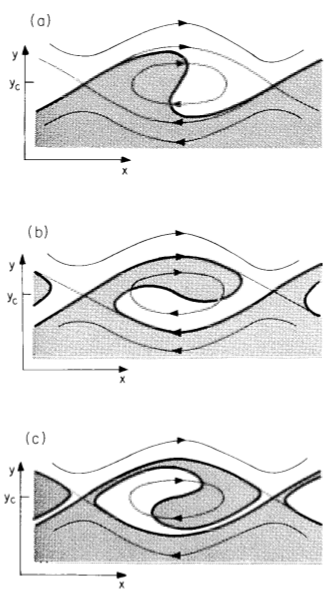
\includegraphics[width=0.5\textwidth]{figures/chapter-intro/breaking_wave_AHL.png}
 \caption[Results from a Stewartson-Warn-Warn model of wave breaking.]{}
 \label{fig:cats_eyes}
\end{figure}

A further effect of wave breaking is the induction of a \emph{residual
  circulation}, $[0, \overline{v}^*, \overline{w}^*]$, where $\overline{v}^*$ and
$\overline{w}^*$ are the transformed Eulerian-mean (TEM) meridional and vertical
velocities given by
\begin{equation}
  \overline{v}^* = \overline{v} - \frac{1}{\rho_0}\frac{\partial}{\partial z}
  \left(\frac{\rho_o\overline{v'\theta'}}{\partial\overline{\theta}/{\partial z}}\right) \, , 
\end{equation}
\begin{equation}
\overline{w}^* = \overline{w} + \frac{1}{a\cos\phi}\frac{\partial}{\partial\phi}
\left(\frac{\cos\phi\overline{v'\theta'}}{\partial\overline{\theta}/{\partial
      z}}\right) \, ,
\end{equation}
which approximate the Lagrangian-mean circulation under time-averaged conditions
\citep{Andrews1976,Dunkerton1978,Holton1980a}. Under the TEM formalism, the zonal
momentum equation becomes
\begin{equation}
\frac{\partial\overline{u}}{\partial t} +
\overline{v}^*\left(\frac{1}{a\cos\phi}\frac{\partial}{\partial\phi}(\overline{u}\cos{\phi})
  - f \right) + \overline{w}^*\frac{\partial\overline{u}}{\partial z} =
\frac{\mathbf{\nabla \cdot F}}{\rho_oa\cos\phi} + \overline{X}
\label{eq:zonal_momentum}
\end{equation}
where $\overline{X}$ represents frictional terms and $\mathbf{F}$ is the
Eliassen-Palm (EP) flux with components
\begin{equation}
F^\phi = \rho_0a\cos\phi\left(\frac{\partial\overline{u}}{\partial
    z}\frac{\overline{v'\theta'}}{\partial\overline{\theta}/\partial z} -
  \overline{v'u'}\right) \, ,
\end{equation}
\begin{equation}
F^z =
\rho_0a\cos\phi\left(\left[f-\frac{1}{a\cos\phi}\frac{\partial}{\partial\phi}(\overline{u}\cos\phi)\right]\frac{\overline{v'\theta'}}{\partial\theta/\partial
      z} - \overline{w'u'}\right) \, .
\end{equation}
$\mathbf{F}$ can be interpreted as the flux of wave activity
\citep{Andrews1987}, and therefore $\mathbf{\nabla\cdot F}<0$ (covergence)
represents a dissipation of wave activity, as is the case in wave breaking. It
can be seen that for a steady zonal flow ($\partial\overline{u}/\partial t = 0$)
in the absence of wave driving ($\mathbf{\nabla\cdot F} = 0$) or friction
($\overline{X} = 0$), a solution of Equation (\ref{eq:zonal_momentum}) is
$\overline{v}^*=0, \overline{w}^*=0$.  However, in the presence of these forcing
terms, a non-zero residual circulation will be induced. Climatologically, this
circulation consists of upwelling in the tropics and poleward and downward
motion in the extratropics; a pattern which forms a significant part of the
Brewer-Dobson circulation\footnote{Strictly, the Brewer-Dobson circulation
  represents the meridional transport of tracers, and so also involves two-way
  mixing.}. The downward motion near the poles can be easily seen from Equation
\ref{eq:zonal_momentum} in the steady case; since $\overline{v}^*$ must become
small near the poles (by conservation of mass), and
$\partial\overline{u}/\partial z > 0$ in the polar vortex, if
$\mathbf{\nabla\cdot F} < 0$, then $\overline{w}^*<0$. It is observed that this
circulation is strongest in the winter hemisphere due to the fact that more
planetary waves can propagate and break in the winter westerly flow than the
summer easterly flow (due to the Charney-Drazin criterion). Furthermore, during
periods of enhanced wave breaking the residual circulation accelerates and there
is more decent and adiabatic heating at high latitudes. This is important in the
physical understanding of sudden stratospheric warming events, described in
Section \ref{sec:strat-sudd-warm}.


\subsubsection{Gravity waves}

Gravity waves are another type of atmospheric wave important in the dynamics of
the polar stratosphere. These waves owe their existence to buoyancy restoring
forces and can be generated by a number of processes such as air flow over
orography (orographic gravity waves), convection or frontogenesis
(non-orographic gravity waves). As with planetary waves, the differences in the
land masses of the two hemispheres leads to orographic gravity wave activity
being much greater in the NH. These waves make a net easterly contribution to
the winter zonal flow \citep[e.g.,][]{Seviour2012}, and so act to enhance the
residual circulation. Their typical length scales are much shorter than can be
resolved in general circulation models or reanalyses, and so they are usually
perameterised, appearing as the term $\overline{X}$ in the zonal momentum
equation (Equation \ref{eq:zonal_momentum}).

\bigskip Together, the Charney-Drazin criterion and the effects of planetary and
gravity wave driving on the zonal flow can expain almost all hemispheric
differences seen in Figures \ref{fig:zmzw_zmT_clim} and \ref{fig:zmzw_NH_SH}:
Greater orography results in more planetary and gravity wave generation in the
NH, both of which cause a net deceleration of the westerly polar vortex, thereby
causing the NH vortex to be weaker than the SH. This also explains why the NH
vortex is warmer than the SH, as the greater NH wave activity induces a stronger
residual circulation with enhanced descent and adiabatic warming at high
latitudes. Additionally, the strength of the SH vortex is such that it prohibits
the vertical propagation of planetary waves from the troposphere throughout much
of the winter, meaning that the SH vortex is less variable than the NH. Both
hemispheres show very little variability in the summer easterly flow because
planetary wave propagation is prohibited in this regime.


\subsection{Sudden stratospheric warmings}
\label{sec:strat-sudd-warm}
%footnote on name
First observed by \citet{Scherhag1952} in radiosonde measurements over Berlin,
the extreme events visible in Figure \ref{fig:zmzw_NH_SH} whereby the winter
circulation temporarily becomes easterly\footnote{For a discussion of more
  precise definitions of SSWs, see Section \ref{sec:moments-introduction}.} are
known as sudden stratospheric warmings\footnote{Following \citet{Butler2014a} it
  is suggested that the term ``sudden stratospheric warming'' is preferrable to
  the common alternative ``stratospheric sudden warming''. This is because there
  are other varieties of stratospheric warming (such as final warmings or
  Canadian warmings), but not other varieties of atmospheric sudden warming.}
(SSWs). These events occur approximately 5-7 times per decade in the NH, but
only one such event has been observed in the $\sim 60$ year observational record
in the SH (in 2002). They are called ``warmings'' because associated with the
circulation reversal is a dramatic increase in temperature; as much as 50~K in
the space of a few days in the midstratosphere.

Initially these events were thought to result from either solar storms or
baroclinic instability of the stratospheric polar vortex. However,
\citet{Matsuno1970, Matsuno1971} proposed a model of SSWs which relies on the
influence of tropospherically forced planetary waves. This model (or
modifications thereof) remains the most widely accepted dynamical view of SSWs
at present. The mechanism proceeds as follows:
\begin{enumerate}[i.]
\item A packet of enhanced planetary wave activity enters the stratosphere where
  it reaches a critical surface and breaks. This decelerates the zonal flow over
  a broader critical layer, and if strong enough causes it to reverse.
\item Hence a new, lower critical surface is formed (where $\overline{u}=0$),
  and wave breaking occurs at this level. The process continues as the critical
  layer descends to the lower stratosphere. 
\item At the same time, wave breaking induces an enhanced residual circulation
  with greater descent and adiabatic warming at high latitudes. If strong
  enough, this can act to reverse the meridional temperature gradient, further
  enhancing the easterly flow by thermal wind balance. 
\item When the critical surface is close to the tropopause, planetary wave
  activity is essentially prohibited from entering the polar
  stratosphere. Radiative cooling to space then acts to cool the polar
  stratosphere and the vortex reforms over a period of approximately 2-4 weeks.
\end{enumerate}

This mechanism takes place in an essentially zonal-mean framework. However, it
has been observed that SSWs generally occur as either a split or displacement of
the vortex, mostly depending (though not exlusively; see Section
\ref{sec:moments-introduction}, \citep{Waugh1997}) on whether wave-2 or wave-1
activity is dominant. An example of each of these events is shown in Figure
\ref{fig:charlton_polvani_ssw}. \citet{Charlton2007a} and \citet{Matthewman2009}
studied the dynamics of these two types of events in reanalysis data and noted
some differences. Most significantly, split vortex events where observed to
occur near-barotropically, with two smaller vortices centred over Canada and
Siberia throughout the depth of the stratosphere. On the other hand, displaced
vortex events were observed to be more baroclinic, starting first in the upper
stratosphere with a vortex centred over Canada, the centre of which rotates
westward with height and is centred over Siberia in the lower stratosphere.


\begin{figure}
 \centering
 \noindent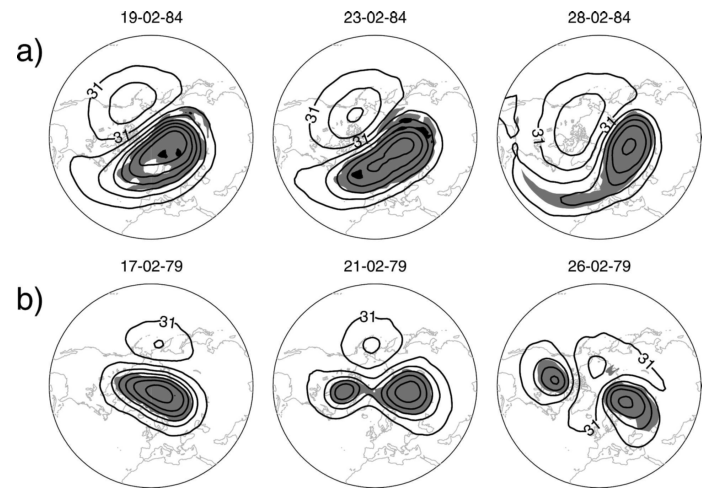
\includegraphics[width=\textwidth]{figures/chapter-intro/charlton_polvani_SSW.png}
 \caption[Examples of a split and displaced vortex event from
 \citet{Charlton2007a}]{Polar stereographic plot of geopotential height
   (contours) on the 10~hPa pressure surface. Contour interval is 0.4~km, and
   shading shows potential vorticity greater than
   $4.0 \times 10^{-6} \mathrm{K~kg^1~m^2~s^{-1}}$. (a) A vortex displacement
   type warming that occurred in February 1984. (b) A vortex splitting type
   warming that occurred in February 1979. From \citet{Charlton2007}.}
 \label{fig:charlton_polvani_ssw}
\end{figure}

This different behaviour of split and displaced vortex events is not accounted
for by the \citet{Matsuno1970, Matsuno1971} model above, and so may suggest that
other mechanisms are important in the generation of SSWs. For instance,
\citet{ONeill1988} and \citet{Scott2006} have suggested that SSWs can be
generated by a cyclone-anticyclone interaction between the Aleutian high and the
polar vortex. These studies showed that a smaller anticyclone can act to
significantly distort the polar vortex, although such interactions are greatest
for circulation ratios higher than are typically found in the polar
stratosphere. Other studies have suggested that SSWs can arise through the
resonant excitation of normal modes of the stratosphere by planetary waves
\citep{Tung1979, Plumb1981, Smith1989}. \citet{Esler2005} and \citet{Esler2006}
suggested that a relevant mode in the case of split vortex events is the
barotropic mode of the atmosphere, which may explain the more barotropic nature
of split vortex events.

Further weight may be given to these mechanisms which do not rely on strong
tropospheric forcing by the ocurrence of the 2002 SH SSW, since this forcing is
much weaker in the SH (several studies of the dynamics of this event can be
found in the March 2005 special issue of \emph{Journal of Atmospheric
  Sciences}). Indeed, \citet{Esler2006} provided evidence that this event may
have been influenced by resonant excitation of the barotropic mode. It should
also be noted that other studies have suggested that SSWs can occur even in the
case of no tropospheric stationary forcing \citep{Kushner2005}.

Overall, while significant advances in understanding the dynamics of SSWs have
been made, several uncertainties remain. While tropospherically-driven wave
activity is certainly an important factor, the roles (if any) of
cyclone-anticyclone interactions or resonance are less certain. Moreover, it is
not clear whether different mechanisms may be more or less important in driving
split and displaced vortex events.


\section{Stratospheric ozone depletion}

The Antarctic ozone is a large region of severely depleted ozone, including the
near-total loss of ozone in the lower stratosphere, which occurs during the
austral spring. A similar, but much smaller depletion is observed in the NH
\citep[e.g.,][]{Manney1996}. Following its discovery by \citet{Farman1985}, a
chemical and dynamical theory of the ozone hole was rapidly developed which is
now widely accepted \citep{McElroy1986,Solomon1986}. This theory is summarised
as follows:
\begin{enumerate}[i.]
\item The strong zonal winds of the stratospheric polar vortex act to confine
  air over the polar regions, with little mixing with midlatitudes
  \citep{Schoeberl1991}. This results in a region of very cold temperatures
  which allow the formation of polar stratospheric clouds (PSCs; these require
  temperatures below approximately 195~K to form).
\item As sunlight returns to the vortex region in spring, hetrogeneous chemical
  rections can take place on the surface of PSCs which act to catalytically
  destroy ozone. The catalysts in these reactions are reactive chlorine and
  bromine species which largely come from anthropogenic chlorofuorocarbons
  (CFCs). 
\item After some time, radiative heating of the stratosphere is sufficient to
  prevent the formation on PSCs, so ozone depletion halts. This heating is
  further accelerated by the increased wave breaking in the polar stratosphere
  which can take place as the vortex weakens (due to the Charney-Drazin
  criterion) and thereby induce an enhanced residual circulation. Following the
  final breakdown of the vortex and transition to easterlies (final warming),
  the ozone-depleted air is mixed to lower latitudes.
\end{enumerate}

\begin{figure}
 \centering
 \noindent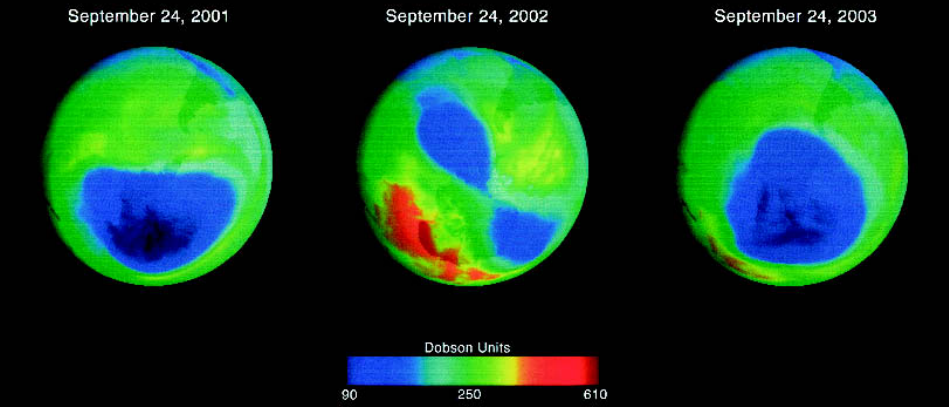
\includegraphics[width=\textwidth]{figures/chapter-intro/2002_SSW.png}
 \caption[]{Comparison of the (middle) first split ozone hole on record (2002)
   and (left) the Antarctic ozone hole at the same time one year earlier (2001)
   and (right) one year later (2003). The hole is dark blue and magenta. In
   2001, the ozone layer thinning over Antarctica reached
   $26.5 \times 10^6~\mathrm{km^2}$ , larger than the size of the entire North
   American continent. Due to higher Antarctic winter temperatures, the 2002
   ``hole'' seems to be about 40\% smaller. In 2003, Antarctic winter
   temperatures returned to normal and the ozone hole returned to its usual
   state. From \citet{Shepherd2005}.}
 \label{fig:2002_SSW}
\end{figure}

Importantly, the stratospheric dynamics described in Section
\ref{sec:dynam-polar-strat}, play an imporant role in ozone depletion. As
discussed in Section \ref{sec:planetary-waves}, wave breaking in the
stratosphere acts to drive a residual circulation, with descent and adiabatic
warming over the pole. Enhanced descent and warming over the pole acts to
inhibit the formation of PSCs which are necessary for the heterogeneous chemical
reactions which cause ozone depletion. 

It is this greater wave activity in the NH then that explains why ozone
depletion is much greater in the SH. Moreover, it has been demonstrated in
interannual variability in wave driving (as measured by
$\mathbf{\nabla\cdot F}$) explains most of the interannual variability of ozone
depletion through this mechanism \citep{Salby2012}. In the extreme event of
SSWs, the ozone hole can be severely disrupted. This can be seen in Figure
\ref{fig:2002_SSW}, where a clear split of the ozone hole is visible during the
2002 SH SSW, which contrasts with the more zonally symmetric distributions seen
at the same times in 2001 and 2003. 

\section{Annular modes}

Before discussing 

\begin{figure}
 \centering
 \noindent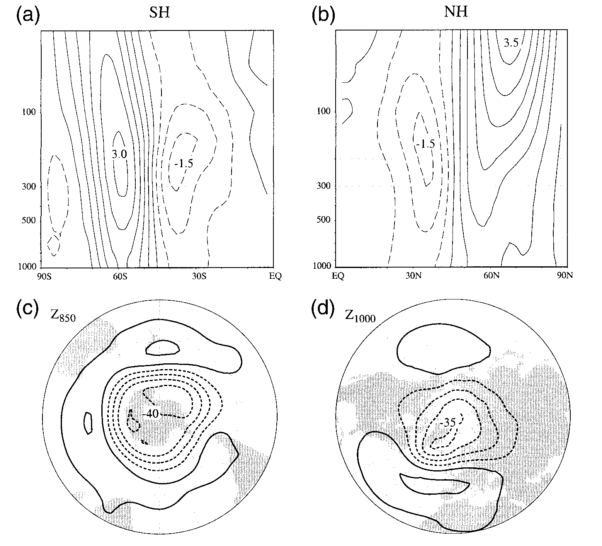
\includegraphics[width=0.6\textwidth]{figures/chapter-intro/annular_modes_TW.png}
 \caption[]{}
 \label{fig:annular_modes}
\end{figure}


\section{Stratosphere-troposphere coupling}
\label{sec:strat-trop-coupl}


\begin{figure}
 \centering
 \noindent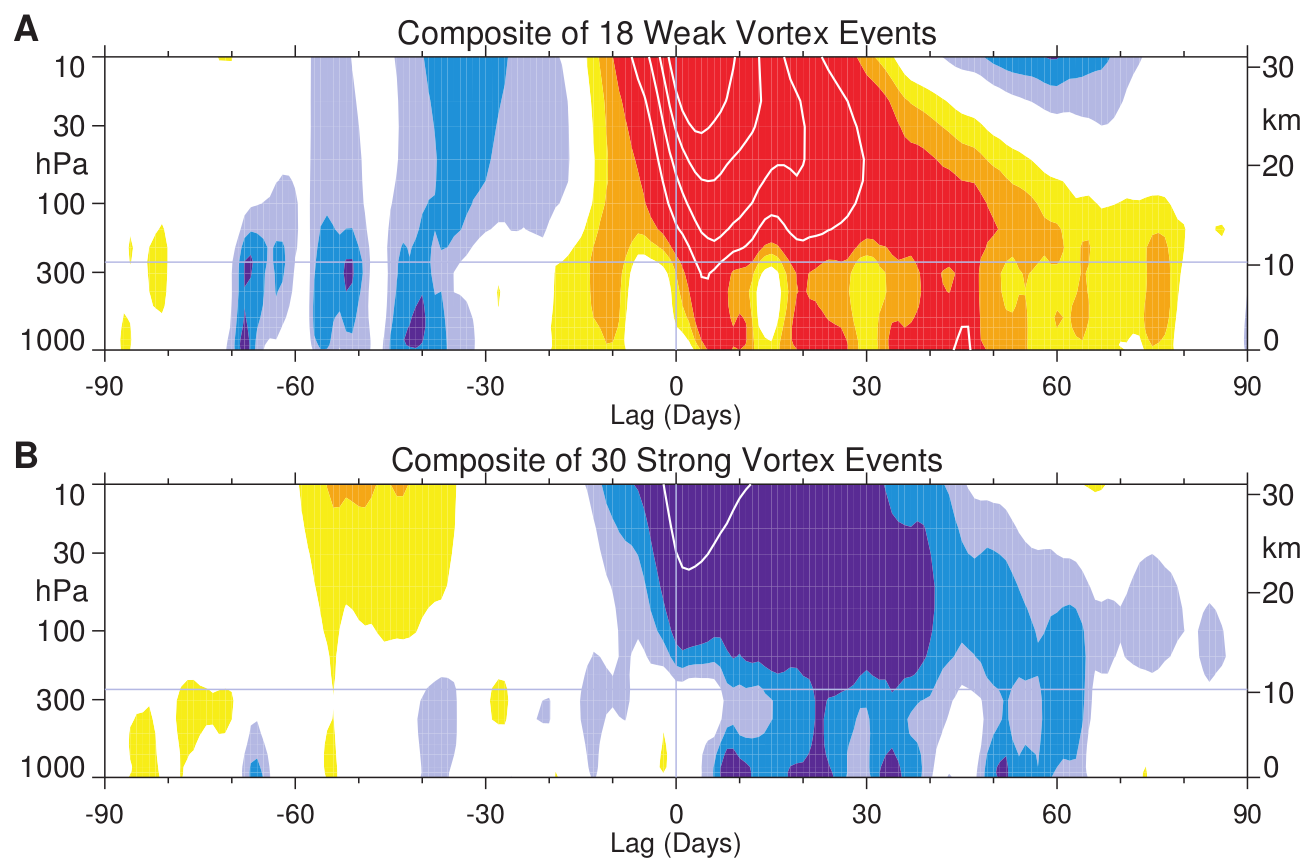
\includegraphics[width=\textwidth]{figures/chapter-intro/Baldwin_Dunkerton.png}
 \caption[NAM composite from \citet{Baldwin2001a}]{Composites of time-height
   development of the northern annular mode for (A) 18 weak vortex events and
   (B) 30 strong vortex events. The events are determined by the dates on which
   the 10-hPa annular mode values cross –3.0 and +1.5, respectively. The indices
   are nondimensional; the contour interval for the color shading is 0.25, and
   0.5 for the white contours. Values between −0.25 and 0.25 are unshaded. The
   thin horizontal lines indicate the approximate boundary between the
   troposphere and the stratosphere. From \citet{Baldwin2001a}.}
 \label{fig:baldwin_dunkerton}
\end{figure}


\subsection{Observational evidence}
\label{sec:observ-evid}
\subsection{Modelling evidence}
\subsection{Mechanisms}
\label{sec:mechanisms}
% Look at Song and Robinson 2004 for basis of mechanisms review
% Radiative Grise, Waugh


\section{Thesis plan}

\begin{figure}
 \centering
 \noindent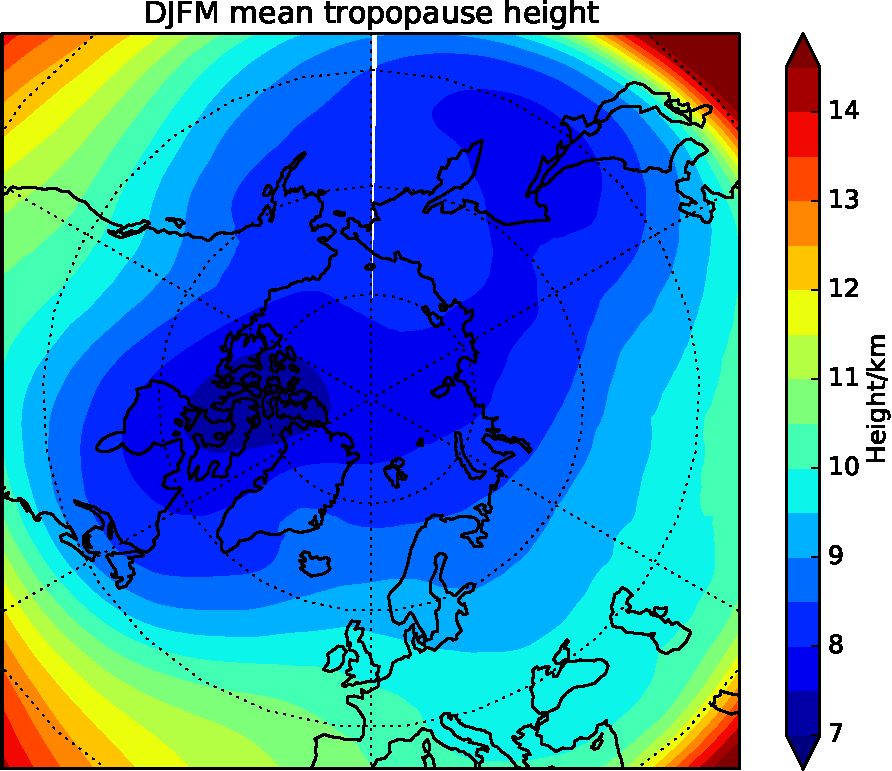
\includegraphics[width=0.5\textwidth]{figures/chapter-intro/mean_tropopause_height.pdf}
 \caption[]{ }
 \label{fig:cmip5_mslp_diff}
\end{figure}



%%% Local Variables:
%%% mode: latex
%%% TeX-master: "thesis"
%%% End:







